
\pgfplotsset{
%        compat=newest,  % <-- does not work; don't know why
        compat=1.13,     % <-- works as expected
    }
  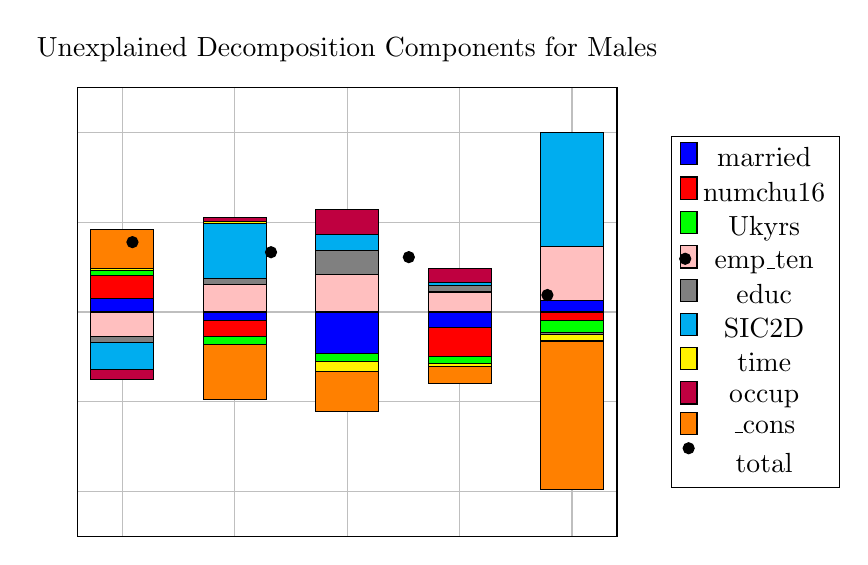
\begin{tikzpicture}
  %\node [align=center, font=\small, rotate=45,text width=2.15cm, inner sep=0.25cm] at (1, 1) {\textsc{year 1}};
  \begin{axis}[
    title={Unexplained Decomposition Components for Males},
    ybar stacked,
    ymax=0.5,
    ymin=-0.5,
    ymajorgrids = true,
    xmajorgrids = true,
    bar width=8mm,
    %xtick={1,2,3,4,5},
    %xticklabels={White, Black, Chinese, Asian, Mixed}
    symbolic x coords={White, Black, Chinese, Asian, Mixed},
    xtick=data,
    nodes near coords align={anchor=north},%Move values in bar
    every node near coord/.style={},
    legend style={at={(1.1,0.5)},anchor=west}
  ]
    %married
    \addplot [fill=blue] coordinates {
({White},0.0297361)
({Black},-0.0186626)
({Chinese},-0.0928553)
({Asian},-0.0342826)
({Mixed},0.0253037)
};
    %numchu16
    \addplot [fill=red] coordinates {
({White},0.0511238)
({Black},-0.035982)
({Chinese},-0.0003413)
({Asian},-0.0643072)
({Mixed},-0.0182561)
};
    %UKyrs
    \addplot [fill=green] coordinates {
({White},0.0118557)
({Black},-0.0182176)
({Chinese},-0.0178013)
({Asian},-0.0159052)
({Mixed},-0.0281895)
};

    %empten
    \addplot [fill=pink] coordinates {
({White},-0.0545902)
({Black},0.0610914)
({Chinese},0.0828618)
({Asian},0.0445577)
({Mixed},0.1204992)
};
    %educ
    \addplot [fill=gray] coordinates {
({White},-0.0137484)
({Black},0.0135428)
({Chinese},0.0536766)
({Asian},0.0154598)
({Mixed},-0.0032165)
};
    %SIC2D
    \addplot [fill=cyan] coordinates {
({White},-0.0598765)
({Black},0.1234811)
({Chinese},0.0355057)
({Asian},0.005262)
({Mixed},0.2540527)
};
    %time
    \addplot [fill=yellow] coordinates {
({White},0.0044796)
({Black},0.0039055)
({Chinese},-0.0209169)
({Asian},-0.0075436)
({Mixed},-0.0149358)
};
    %occup
    \addplot [fill=purple] coordinates {
({White},-0.0220507)
({Black},0.0084218)
({Chinese},0.0569902)
({Asian},0.0321543)
({Mixed},0.0000381)
};
    %_cons
    \addplot [fill=orange] coordinates {
({White},0.0865697)
({Black},-0.1223497)
({Chinese},-0.0908395)
({Asian},-0.0378478)
({Mixed},-0.331977)
};
\addplot [only marks,mark=*,mark size=2pt,black,
         nodes near coords = \rotatebox{90}{{\pgfmathprintnumber[fixed zerofill,
                                    precision=2]{\pgfplotspointmeta}}},
        nodes near coords align={vertical},
        point meta=y,
        every node near coord/.append style={font=\small, yshift=0.25mm},] coordinates {({Mixed},-1)};
%\begin{comment}
%\end{comment}
%\filldraw[black] (0,0) circle (2pt) node[anchor=west] {Intersection point};
  \legend{married, numchu16, Ukyrs, emp\_ten, educ, SIC2D, time, occup, \_cons, total}
  \end{axis}
  
  \begin{axis}[
    nodes near coords align={anchor=north},%Move values in bar
    every node near coord/.style={},
    xtick=data,
    ymax=0.3,
    ymin=-0.3,
    xmax=0,
    xmin=5,
]
\pgfplotsset{ticks=none}
\addplot[only marks,mark=*,mark size=3pt,black,
         nodes near coords = \rotatebox{90}{{\pgfmathprintnumber[fixed zerofill,
                                    precision=2]{\pgfplotspointmeta}}},
        nodes near coords align={vertical},
        point meta=y,
        every node near coord/.append style={font=\small, yshift=0.25mm},
        ]  coordinates {
    (1,0.1) (2,-0.1) (3,1)
};
\end{axis}
\filldraw[black] (0.7,3.7344923) circle (2pt) node[anchor=west] {};
\filldraw[black] (2.46,3.6066156) circle (2pt) node[anchor=west] {};
\filldraw[black] (4.21,3.5439593) circle (2pt) node[anchor=west] {};
\filldraw[black] (5.97,3.0628304) circle (2pt) node[anchor=west] {};
\filldraw[black] (7.72,3.5232309) circle (2pt) node[anchor=west] {};
  \end{tikzpicture}
